\documentclass[a4paper]{IEEEtran}
\usepackage{amsmath}
\renewcommand\IEEEkeywordsname{Kata Kunci}
\usepackage[bahasa]{babel}
\addto{\captionsbahasa}{\renewcommand{\abstractname}{Abstrak}}
\addto{\captionsbahasa}{\renewcommand*{\refname}{DAFTAR PUSTAKA}
}
\usepackage[utf8]{inputenc}
\usepackage{caption}
\usepackage{graphicx}
\usepackage{hyperref}
\usepackage{xesearch}

% Table caption above table
\usepackage{float}
\floatstyle{plaintop}
\restylefloat{table}

% Centering table caption
\usepackage[justification=centering]{caption}

% Prevent hyphenation
\usepackage[none]{hyphenat}


\setcounter{table}{0}
\renewcommand{\thetable}{\arabic{table}}
\renewcommand{\thefigure}{\arabic{figure}}

\usepackage{caption}
\captionsetup[table]{labelsep=space}
\captionsetup[figure]{labelsep=space}
\captionsetup[lstlisting]{labelsep=space}

\markboth{\normalsize JURNAL TEKNIK ITS Vol. 4, No. 1, (2015) ISSN: 2337-3539 (2301-9271 Print)}{}
\begin{document}
\title{Desain, Analisis dan Implementasi Algoritma Komputasi String dengan Metode Dynamic Programming dan Meet In the Middle pada Permasalahan Klasik SPOJ 9967 Playing With Words}
\author{\IEEEauthorblockN{Dewangga Winasforcepta Winardi, Rully Soelaiman dan F. X. Arunanto}\\
\IEEEauthorblockA{Departemen Teknik Informatika, Fakultas Teknologi Informasi, Institut Teknologi Sepuluh Nopember (ITS)\\
Jl. Arief Rahman Hakim, Surabaya 60111 Indonesia\\
e-mail: dewangga13@mhs.if.its.ac.id, rully@is.its.ac.id, anto@if.its.ac.id}}
\maketitle

% ABSTRAK
\begin{abstract}
	 Diberikan dua buah \textit{string} $orig1$ dan $orig2$. Diberikan tiga tahapan proses transformasi untuk menghasilkan \textit{string} $ad1$ dan $ad2$. Tahap pertama adalah \textit{string} $orig1$ diacak urutan karakter-karakternya. Tahap kedua adalah \textit{string} $orig2$ diacak urutan karakter-karakternya. Tahap terakhir adalah salah satu karakter dari \textit{string} $orig1$ atau $orig2$ diganti dengan karakter sebelum atau sesudahnya dalam alfabet. Jarak dua buah \textit{string} didefinisikan sebagai jumlah dari selisih mutlak dari karakter-karakter pada posisi yang sama. Diberikan sebuah bilangan bulat $X$ yang merupakan jarak dari \textit{string} $orig1$ dan \textit{string} $ad1$ dijumlahkan dengan jarak dari \textit{string} $orig2$ dan \textit{string} $ad2$. Tentukan jumlah kemungkinan kombinasi \textit{string} $orig1$ dan $orig2$ jika diberikan \textit{string} $ad1$, $ad2$ dan nilai $X$.	 
	 
	 Pada penelitian ini akan dirancang penyelesaian masalah yang disampaikan pada paragraf pertama dengan menggunakan pendekatan \textit{dynamic programming} dan teknik \textit{meet in the middle}. Solusi yang dikembangkan berjalan dengan kompleksitas waktu $\mathcal{O}(2^{|S|} * MAX\_DIST^{2} * T)$, di mana $|S|$ adalah panjang \textit{string} yang diberikan dan $MAX\_DIST$ adalah jarak antar \textit{string} maksimal.
	 
	 Algoritma yang dirancang dapat menyelesaikan permasalahan yang diberikan dengan benar. Pada kasus terburuk, waktu eksekusi program yang mengimplementasi algoritma yang dirancang tidak melebihi batas waktu eksekusi program yang telah diberikan, yaitu $ 6,459 $ detik. Sehingga dapat disimpulkan algoritma yang dibangun dapat menyelesaikan permasalahan yang diberikan.
\end{abstract}
\begin{IEEEkeywords}
	\textit{string}, \textit{divide and conquer}, \textit{meet in the middle}, \textit{dynamic programming}
\end{IEEEkeywords}

\section{PENDAHULUAN}

Diberikan dua buah \textit{string} $orig1$ dan $orig2$. Diberikan tiga tahapan proses transformasi untuk menghasilkan \textit{string} $ad1$ dan $ad2$ sebagai berikut:

\begin{enumerate}
	\item String $orig1$ diacak urutan karakter-karakternya.
	\item String $orig2$ diacak urutan karakter-karakternya.
	\item Salah satu karakter dari \textit{string} $orig1$ atau $orig2$ diganti dengan karakter sebelum atau sesudahnya dalam alfabet.
\end{enumerate}	

Jarak dua buah \textit{string} didefinisikan sebagai jumlah dari selisih mutlak dari karakter-karakter pada posisi yang sama. Diberikan sebuah bilangan bulat $X$ yang merupakan jarak dari \textit{string} $orig1$ dan \textit{string} $ad1$ dijumlahkan dengan jarak dari \textit{string} $orig2$ dan \textit{string} $ad2$. Berapakah jumlah kemungkinan kombinasi \textit{string} $orig1$ dan $orig2$ jika diberikan \textit{string} $ad1$, $ad2$ dan nilai $X$.

Solusi naif dari permasalahan di atas adalah dengan mengkomputasi semua kemungkinan \textit{string} $ orig1 $ dan $ orig2 $ lalu menghitung berapa banyak kombinasi \textit{string} $ orig1 $ dan $ orig2 $ yang memiliki $ dist(orig1, ad1) + dist(orig2, ad2) = X $. Namun solusi tersebut tentu akan membutuhkan waktu komputasi yang sangat besar. Permasalahan di atas dapat dipecah menjadi beberapa submasalah yang memiliki karakteristik tidak memiliki ketergantungan satu sama lain dengan menghitung jumlah kombinasi untuk masing-masing \textit{string} $ ad1 $ dan $ ad2 $. Sehingga pendekatan \textit{divide and conquer} dengan teknik \textit{meet in the middle} dapat diaplikasikan pada permasalahan ini. Setiap submasalah dapat dipecah menjadi submasalahan-submasalah yang memiliki karakteristik saling tumpang tindih. Sehingga, pendekatan \textit{dynamic programming} dapat dimanfaatkan untuk menyelesaikan setiap submasalah sebelum solusi setiap submasalah digabungkan untuk membentuk jawaban akhir. Tujuan dari penelitian ini adalah untuk menyelesaikan permasalahan, menguji kebenaran dan menguji performa dari algoritma yang dibangun.

\section{METODE PENYELESAIAN}


Untuk merancang algoritma yang optimal untuk menyelesaikan permasalahan yang diberikan, dapat dilakukan penyelesaian permasalahan yang lebih sederhana. Awalnya, diasumsikan tidak ada operasi \textit{replace} untuk mentransformasi pesan asli menjadi kalimat iklan. Gambar \ref{figure:algo1} adalah algoritma untuk menghitung jumlah kemungkinan pesan asli dari pesan iklan yang diberikan. Contohnya ketika kalimat pesan adalah $ ad1=bc $, \textit{string} $ ad2=efg $ dan $ X=4 $. Setelah mencari seluruh kombinasi \textit{string} $ orig1 $ dari \textit{string} $ ad1 $ dan \textit{string} $ orig2 $ dari \textit{string} $ ad2 $ beserta jarak masing-masing, setiap kombinasi \textit{string} $ orig1 $ dengan jarak $ D $ dipasangkan dengan setiap \textit{string} $ orig2 $ dengan jarak $ X-D $ dengan $ 0 \le D \le X $. Tabel \ref{tab:algo1} menunjukkan bahwa terdapat $ 5 $ kombinasi pesan asli dari pesan iklan dengan \textit{string} $ ad1=bc $, \textit{string} $ ad2=efg $ dan $ X=4 $.

\begin{figure}[h]
	\centering
	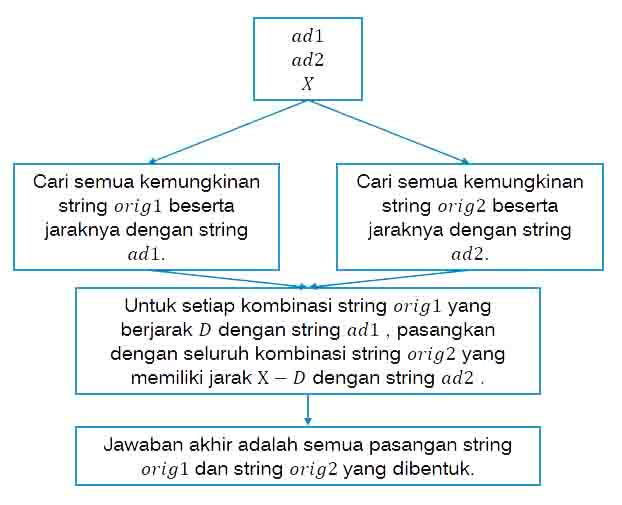
\includegraphics[width=\linewidth]{images/algo1.jpg}
	\caption{Algoritma komputasi jumlah kombinasi \textit{string} $ orig $ tanpa operasi \textit{replace}}
	\label{figure:algo1}
\end{figure}

\begin{table}
	\centering
	\begin{tabular} {|p{1cm}|p{2.5cm}|p{1cm}|p{2.5cm}|} \hline
		$ orig1 $ & $ dist(orig1, ad1) $ & $ orig2 $ & $ dist(orig2, ad2) $ \\ \hline
		$ bc $ & $ 0 $ & $ feg $ & $ 4 $ \\ \hline		
		$ bc $ & $ 0 $ & $ gef $ & $ 4 $ \\ \hline
		$ bc $ & $ 0 $ & $ gfe $ & $ 4 $ \\ \hline
		$ cb $ & $ 2 $ & $ egf $ & $ 2 $ \\ \hline
		$ cb $ & $ 2 $ & $ fge $ & $ 2 $ \\ \hline
	\end{tabular}\caption{Kombinasi \textit{string} $ orig1 $ dan \textit{string} $ orig2 $ dari \textit{string} $ ad1=bc $ dan \textit{string} $ ad2= efg$ tanpa operasi \textit{replace} dengan $ X=4$} 
	\label{tab:algo1}
\end{table}


Algoritma pada Gambar \ref{figure:algo2} adalah algoritma untuk mencari kombinasi pesan asli dari pesan iklan dengan sekali operasi \textit{replace} sesuai pada deskripsi permasalahan. Contohnya ketika kalimat pesan adalah $ ad1=c $, \textit{string} $ ad2=n $ dan $ X=1 $. Hasil didapatkan dengan dua perhitungan yaitu perhitungan jumlah kombinasi \textit{string} $ orig1 $ tanpa operasi \textit{replace} dengan jarak $ D $ terhadap \textit{string} $ ad1 $ yang dipasangkan dengan setiap kombinasi \textit{string} $ orig2 $ dengan sekali operasi \textit{replace} dengan jarak $ X-D $ terhadap \textit{string} $ ad2 $. Berikutnya jawaban ditambahkan dengan hasil perhitungan kedua yaitu perhitungan jumlah kombinasi \textit{string} $ orig1 $ dengan sekali operasi \textit{replace} dengan jarak $ D $ terhadap \textit{string} $ ad1 $ yang dipasangkan dengan setiap kombinasi \textit{string} $ orig2 $ tanpa operasi \textit{replace} dengan jarak $ X-D $ terhadap \textit{string} $ ad2 $. Tabel \ref{tab:algo2} menunjukkan bahwa terdapat $ 4 $ kombinasi pesan asli dari pesan iklan dengan \textit{string} $ ad1=c $, \textit{string} $ ad2=n $ dan $ X=1 $.

\begin{figure}[h]
	\centering
	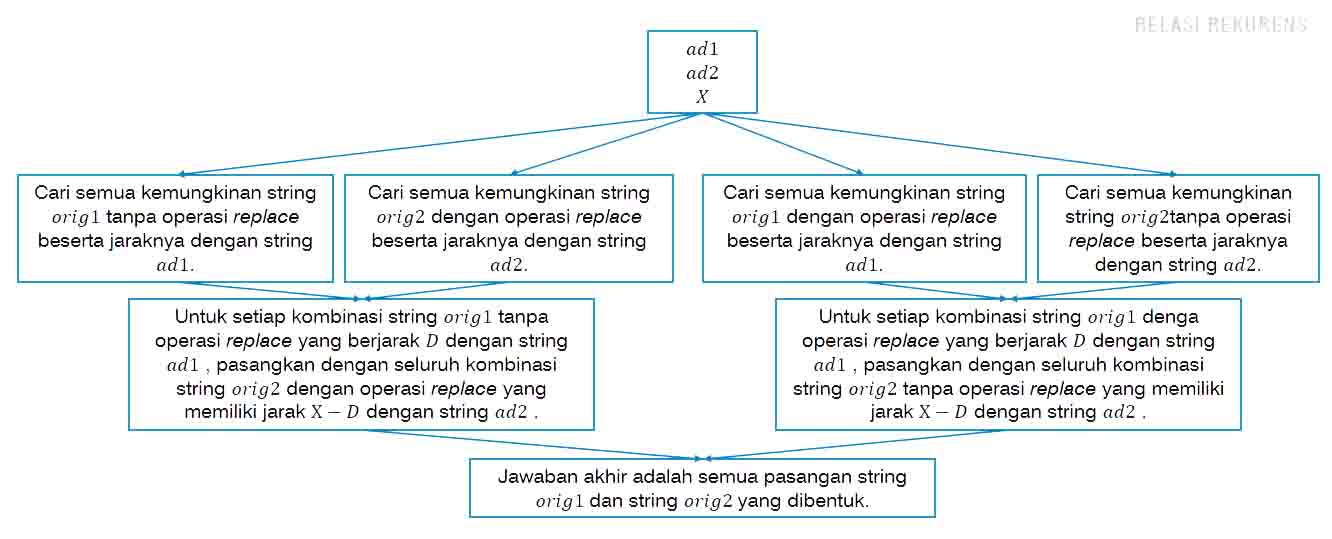
\includegraphics[width=\linewidth]{images/algo2.jpg}
	\caption{Algoritma komputasi jumlah kombinasi \textit{string} $ orig $ tanpa operasi \textit{replace}}
	\label{figure:algo2}
\end{figure}

\begin{table}
	\centering
	\begin{tabular} {|p{1cm}|p{2.5cm}|p{1cm}|p{2.5cm}|} \hline
		$ orig1 $ & $ dist(orig1, ad1) $ & $ orig2 $ & $ dist(orig2, ad2) $ \\ \hline
		$ c $ & $ 0 $ & $ m $ & $ 1 $ \\ \hline		
		$ c $ & $ 0 $ & $ o $ & $ 1 $ \\ \hline
		$ b $ & $ 1 $ & $ n $ & $ 0 $ \\ \hline
		$ d $ & $ 1 $ & $ n $ & $ 0 $ \\ \hline
	\end{tabular}\caption{Kombinasi \textit{string} $ orig1 $ dan \textit{string} $ orig2 $ dari \textit{string} $ ad1=c $ dan \textit{string} $ ad2= n$ dengan sekali operasi \textit{replace} dengan $ X=1$} 
	\label{tab:algo2}
\end{table}


Pada permasalahan tidak diperlukan informasi kombinasi pesan asli yang mungkin, melainkan hanya memerlukan informasi jumlah kemungkinan kombinasi pesan asli yang mungkin. Sehingga algoritma komputasi dapat dioptimasi menjadi lebih efisien. Gambar \ref{figure:algo3} adalah algoritma yang optimal untuk menghitung jumlah kemungkinan pesan asli dari pesan iklan. Contohnya pada kasus ketika kalimat pesan adalah $ ad1=c $, \textit{string} $ ad2=n $ dan $ X=1 $. Algoritma pada Gambar \ref{figure:algo3} mirip dengan algoritma pada Gambar \ref{figure:algo2}. Hanya saja pada algoritma ini tidak dicari semua kemungkinan \textit{string} $ orig $, hanya dihitung kemungkinannya saja. Contohnya pada perhitungan kemungkinan \textit{string} $ orig1 $ dari \textit{string} $ ad1=c $. Algoritma hanya menghitung jumlah kombinasi \textit{string} $ orig1 $ tanpa operasi \textit{replace} dengan jarak $ 0 $ dan $ 1 $ terhadap \textit{string} $ ad1 $ seperti yang terlihat pada Tabel \ref{tab:algo3_1}. Hasil akhir perhitungan adalah terdapat $ 4 $ kombinasi pesan asli seperti yang terlihat pada Tabel \ref{tab:algo3_2}.

\begin{table}
	\centering
	\begin{tabular} {|p{2cm}|p{3cm}|} \hline
		$ D $ & Jumlah kombinasi \textit{string} $ orig1 $\\ \hline
		$ 0 $ & $ 1 $ \\ \hline		
		$ 1 $ & $ 0 $ \\ \hline
	\end{tabular}\caption{Hasil perhitungan jumlah kombinasi \textit{string} $ orig1 $ tanpa operasi \textit{replace} dengan jarak $ 0 $ dan $ 1 $ terhadap \textit{string} $ ad1 $} 
	\label{tab:algo3_1}
\end{table}

\begin{table}
	\centering
	\begin{tabular} {|p{1cm}|p{1.65cm}|p{1cm}|p{1.65cm}|p{0.5cm}|} \hline
		$ D $ & Jumlah kombinasi \textit{string} $ orig1 $ & $ X-D $ & Jumlah kombinasi \textit{string} $ orig2 $ & total \\ \hline
		$ 0 $ & $ 1 $ & $ 1 $ & $ 2 $ & $ 2 $ \\ \hline		
		$ 1 $ & $ 0 $ & $ 0 $ & $ 0 $ & $ 0 $ \\ \hline
		$ 0 $ & $ 0 $ & $ 1 $ & $ 1 $ & $ 0 $ \\ \hline
		$ 1 $ & $ 2 $ & $ 0 $ & $ 1 $ & $ 2 $ \\ \hline
	\end{tabular}\caption{Kombinasi \textit{string} $ orig1 $ dan \textit{string} $ orig2 $ dari \textit{string} $ ad1=c $ dan \textit{string} $ ad2= n$ dengan sekali operasi \textit{replace} dengan $ X=1$} 
	\label{tab:algo3_2}
\end{table}

\begin{figure}[h]
	\centering
	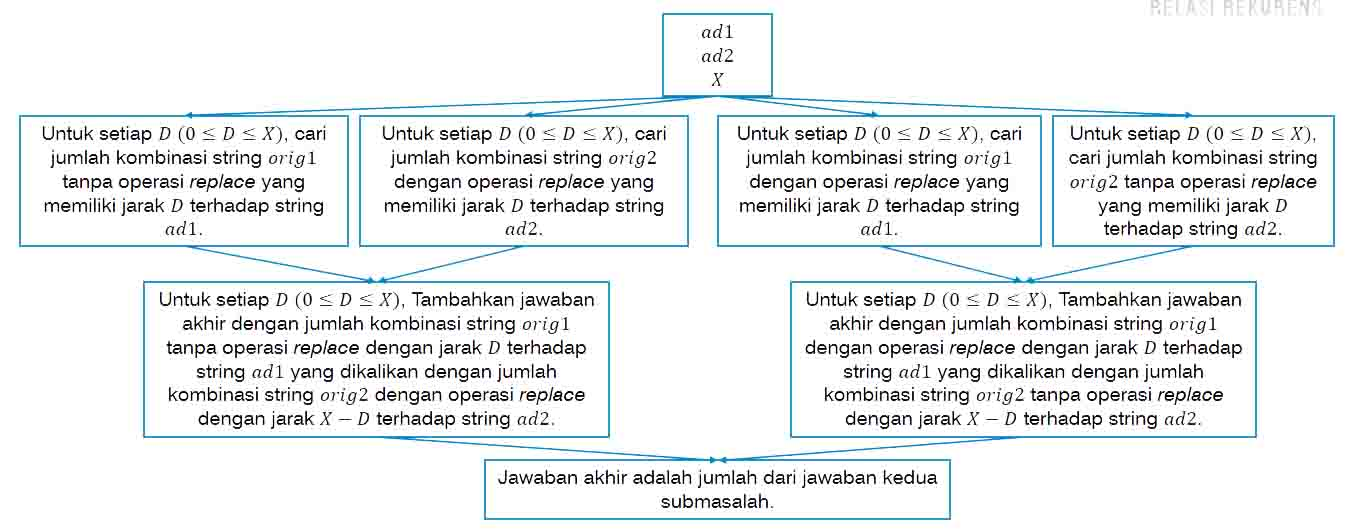
\includegraphics[width=\linewidth]{images/algo3.jpg}
	\caption{Algoritma komputasi jumlah kombinasi \textit{string} $ orig $ tanpa operasi \textit{replace}}
	\label{figure:algo3}
\end{figure}

\begin{equation}
answer = \parbox[t]{0.8\linewidth}{ $\sum_{dist=0}^{dist=min_{(X, 250)}}((F_{(S_{0}, 2^{|S_{0}|}, bound - dist)} * G_{(S_{1}, 2^{|S_{1}|}, bound - X + dist)}) + (G_{(S_{0}, 2^{|S_{0}|}, bound -dist)} * F_{(S_{1},2^{|S_{1}|},bound-X+dist)}))$}
\label{equation:main_answer}
\end{equation}


\begin{equation}
F_{(S,mask,dist)}= 
\begin{cases}
0,& \text{if }  \parbox[t]{0.3\linewidth} {$ dist > bound \vee (mask=0 \wedge dist \neq bound) $} \\
1,& \text{if }  \parbox[t]{0.3\linewidth} {$(mask=0) \wedge (dist=bound)$} \\
\parbox[t]{0.3\linewidth}{$ \sum_{i=0}^{i=NSB_{(mask)}} \\F1_{(S, mask,
		set\_bit(mask)_{i}, dist)} $}& \text{otherwise}
\end{cases}
\label{equation:rekurens_f}
\end{equation}


\begin{equation}
G_{(S,mask,dist)}= 
\begin{cases}
0,& \text{if }  \parbox[t]{0.3\linewidth} {$ (dist > bound) \vee mask = bound$} \\
\parbox[t]{0.3\linewidth}{$ \sum_{i=0}^{i=NSB_{(mask)}} \\G1_{(S, mask,
		set\_bit(mask)_{i}, dist)}\\+G2_{(S, mask,
		set\_bit(mask)_{i}, dist)}\\+G3_{(S, mask,
		set\_bit(mask)_{i}, dist)} $}& \text{otherwise}
\end{cases}
\label{equation:rekurens_g}
\end{equation}

\begin{equation*}
F1_{(S,mask,idx,dist)}= 
\begin{cases}
\parbox[t]{0.25\linewidth}{$ F_{(S, mask - 2^{idx}, dist +}\\_{|S_{idx} - S_{curIdx}|)} $}& \text{if } \parbox[t]{0.3\linewidth}{$idx = |S| - 1 \vee duplicate\_rule1\\_{(S, mask, idx)} = True$}\\
0,& \text{otherwise}
\end{cases}
\end{equation*}

\begin{equation*}
G1_{(S,mask,idx,dist)}= 
\begin{cases}
\parbox[t]{0.25\linewidth}{$ G_{(S, mask - 2^{idx}, dist +}\\_{|S_{idx} - S_{curIdx}|)} $}& \text{if } \parbox[t]{0.3\linewidth}{$idx=|S|-1 \vee duplicate\_rule1\\_{(S, mask, idx)} = True$}\\
0,& \text{otherwise}
\end{cases}
\end{equation*}

\begin{equation*}
G2_{(S,mask,idx, dist)}= 
\begin{cases}
\parbox[t]{0.25\linewidth}{$ F\\_{(S, mask - 2^{idx}, dist +}\\_{|S_{idx}+1 - S_{curIdx}|)} $}& \text{if } \parbox[t]{0.25\linewidth}{$idx=|S|-1 \vee (duplicate\_rule1\\_{(S, mask, idx)} = True \wedge duplicate\_rule2\\_{(S, mask, idx)} = True)$}\\
0,& \text{otherwise}
\end{cases}
\end{equation*}

\begin{equation*}
G3_{(S,mask,idx, dist)}= 
\begin{cases}
\parbox[t]{0.25\linewidth}{$ F\\_{(S, mask - 2^{idx}, dist +}\\_{|S_{idx}-1 - S_{curIdx}|)} $}& \text{if } \parbox[t]{0.25\linewidth}{($idx=|S|-1 \vee duplicate\_rule1\\_{(S, mask, idx)} = True) \wedge (idx=0 \vee duplicate\_rule3\\_{(S, mask, idx)} = True)$}\\
0,& \text{otherwise}
\end{cases}
\end{equation*}

\begin{equation*}
\parbox[t]{0.3\linewidth}{$ duplicate\_rule1\\_{(S,mask,dist)}=  $}
\begin{cases}
True& \text{if } \parbox[t]{0.3\linewidth}{$idx < |S| -1 \wedge (S_{idx} \neq S_{idx + 1}  \vee ((S_{idx} = S_{idx + 1})  \wedge (is\_on_{(mask, idx + 1)} =  False$))}\\
False,& \text{otherwise}
\end{cases}
\end{equation*}

\begin{equation*}
\parbox[t]{0.3\linewidth}{$ duplicate\_rule2\\_{(S,mask,dist)}=  $}
\begin{cases}
True& \text{if } \parbox[t]{0.3\linewidth}{$idx < |S| -1
	\wedge (charFirstPos\\_{(S, S_{idx} + 1)} = -1
	\vee (charFirstPos\\_{(S, S_{idx} + 1)} \neq -1 
	\wedge is\_on_{(mask}\\_{charFirstPos}\\_{_{(S, S_{idx} + 1)})} = False$}\\
False,& \text{otherwise}
\end{cases}
\end{equation*}

\begin{equation*}
\parbox[t]{0.3\linewidth}{$ duplicate\_rule3\\_{(S,mask,dist)}=  $}
\begin{cases}
True& \text{if } \parbox[t]{0.25\linewidth}{$idx > 0 -1
	\wedge (charLastPos_{(S,}\\_{S_{idx} - 1)} = -1
	\vee (charLastPos_{(S, }\\_{S_{idx} - 1)} \neq -1 
	\wedge is\_on_{(mask,}\\_{ charLastPos}\\_{_{(S, S_{idx} - 1)})}=True$}\\
False,& \text{otherwise}
\end{cases}
\end{equation*}

\begin{equation*}
is\_on_{(mask, idx)} =
\begin{cases}
True& \text{if } \parbox[t]{0.3\linewidth}{($mask \& 2^{idx}) = 1$}\\
False,& \text{otherwise}
\end{cases}
\end{equation*}

\begin{table}
	\centering
	\begin{tabular} {|p{3cm}|p{5cm}|} \hline
		Notasi & Deskripsi\\ \hline
		$ S $ & String yang akan dicari kemungkinan \textit{string} awalnya.\\ \hline
		$ mask $ & Sebuah bilangan bulat yang bertugas sebagai \textit{bitmask} yang merepresentasikan kondisi karakter mana saja yang sudah diambil pada kondisi (\textit{state}) tersebut.\\ \hline
		$ dist $ & Jarak \textit{string} yang sudah terbentuk pada kondisi tersebut dengan \textit{string} $ S $ dari $ bound $ atau secara matematis dapat dituliskan dengan $ bound - distance(currentString, S) $.\\ \hline
		$ bound $ & Nilai batas jarak maksimal yang bernilai $ min(X, 250) $\\ \hline
		$ idx $ & Index karakter pada \textit{string} $ S $ yang akan diambil atau digunakan.\\ \hline
		$ NSB_{(mask)} $ & Mengembalikan jumlah angka 1 pada $ mask $ apabila direpresentasikan dalam basis biner\\ \hline
		$ set\_bit_{(mask)} $ & Himpunan index bilangan bernilai satu dari $ mask $ apabila direpresentasikan dalam basis biner.\\ \hline
		$ is\_on_{(mask, idx)} $ & Mengembalikan nilai $ true $ apabila bilangan pada index $ idx $ pada $ mask $ dalam basis biner bernilai $ 1 $.\\ \hline
		$ charLastPos_{(S, C)} $ & Index terbesar dari karakter $ C $ pada \textit{string} $ S $.\\ \hline
		$ charFirstPos_{(S, C)} $ & Index terkecil dari karakter $ C $ pada \textit{string} $ S $.\\ \hline
		$ curIdx $ & Angka yang merepresentasikan panjang \textit{string} $ orig $ pada \textit{state} tersebut. Nilai $ curIdx $ adalah jumlah bit yang bernilai $ 0 $ pada $ mask $.\\ \hline
	\end{tabular}\caption{Daftar notasi persamaan relasi rekurens}
	\label{tab:daftar_notasi}
\end{table}

Persamaan \ref{equation:main_answer} adalah persamaan untuk mendapatkan jawaban akhir dengan fungsi $ F_{(S, mask, idx)} $ pada Persamaan \ref{equation:rekurens_f} adalah fungsi untuk menghitung kemungkinan kombinasi \textit{string} $ orig $ dari \textit{string} $ S $ tanpa operasi \textit{replace} dan fungsi $ G_{(S, mask, idx)} $ adalah fungsi untuk menghitung kemungkinan kombinasi \textit{string} $ orig $ dari \textit{string} $ S $ dengan sekali operasi \textit{replace}. Tabel \ref{tab:daftar_notasi} adalah daftar notasi dari persamaan-persamaan tersebut.

\section{UJI COBA DAN ANALISIS}



\subsection{Uji coba kebenaran}
Uji coba kebenaran dilakukan dengan mengumpulkan berkas kode sumber hasil implementasi ke situs sistem penilaian daring SPOJ kali. Permasalahan yang diselesaikan adalah Playing With Words dengan kode PWORDS. Hasil uji kebenaran dan waktu eksekusi program saat pengumpulan kasus uji pada situs SPOJ ditunjukkan pada Gambar \ref{figure:uji_kebenaran_spoj}.

\begin{figure}[h]
	\centering
	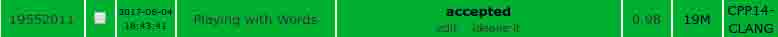
\includegraphics[width=\linewidth]{images/single-submission.jpg}
	\caption{Hasil uji kebenaran dengan melakukan \textit{submission} ke situs penilaian daring SPOJ}
	\label{figure:uji_kebenaran_spoj}
\end{figure}

Berikutnya adalah pengujian performa dari algoritma yang dirancang dan diimplementasi dengan melakukan uji \textit{submission} dengan mengumpulkan berkas kode implementasi dari algoritma yang dibangun sebanyak 30 kali ke situs penilaian daring SPOJ dengan mencatat waktu eksekusi serta memori yang dibutuhkan. Hasil dari pengujian dapat dilihat pada grafik pada Gambar \ref{figure:chart} dan Tabel \ref{tab:statistik}.

\begin{figure}[h]
	\centering
	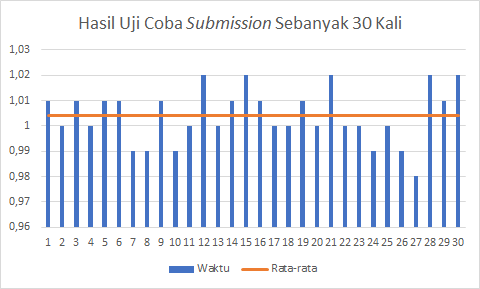
\includegraphics[width=\linewidth]{submission-chart.png}
	\caption{Hasil Uji Coba \textit{Submission} ke situs penilaian daring SPOJ sebanyak 30 kali}
	\label{figure:chart}
\end{figure}

\begin{table}
	\centering
	\begin{tabular}{|l|l|} \hline
		Waktu Maksimal & $ 1.02 $ detik\\ \hline
		Waktu Minimal & $ 0.98 $ detik\\ \hline
		Waktu Rata-Rata & $ 1.004 $ detik\\ \hline
		Memori Maksimal & $ 19 $ MB\\ \hline
		Memori Minimal & $ 19 $ MB\\ \hline
		Memori Rata-Rata & $ 19 $ MB\\ \hline
	\end{tabular}
	\caption{Kecepatan maksimal, minimal dan rata-rata dari hasil uji coba pengumpulan 30 kali pada situs pengujian daring SPOJ}
	\label{tab:statistik}
\end{table}


\subsection{Analisis Kompleksitas}
Berdasarkan Persamaan \ref{equation:main_answer} didapatkan algoritma dengan kompleksitas waktu $ \mathcal{O}(2^{|S|} * MAX\_DIST^{2} * T) $ di mana $ |S| $ adalah panjang \textit{string} masukan, $ MAX\_DIST^{2} $ adalah jarak maksimal antar \textit{string} dan $ T $ adalah banyaknya kasus uji. Pada umumnya, eksekusi program pada situs penilaian daring SPOJ adalah $ 1 $ detik untuk setiap $ 100.000.000 $ proses. Pada kasus terburuk, yaitu ketika $ |S|=10 $, $ MAX\_DIST=250 $ dan $ T=10 $, eksekusi program dengan kompleksitas waktu $ \mathcal{O}(2^{|S|} * MAX\_DIST^{2} * T) $ akan melakukan $ 640.000.000 $ proses di mana jika dengan menggunakan standar berupa $ 100.000.000 $ proses per detik, program akan membutuhkan waktu eksekusi sebesar $ 6,4 $ detik. Sehingga Algoritma dengan kompleksitas waktu $ \mathcal{O}(2^{|S|} * MAX\_DIST^{2} * T) $ dapat menyelesaikan permasalahan yang diberikan.


\section{KESIMPULAN}

Dari hasil uji coba yang telah dilakukan terhadap perancangan dan implementasi algoritma untuk menyelesaikan permasalahan klasik SPOJ 9967 Playing With Words dapat diambil kesimpulan sebagai berikut:

\begin{enumerate}
	\item Implementasi algoritma dengan menggunakan pendekatan \textit{dynamic programming} dan teknik \textit{meet in the middle} dapat menyelesaikan permasalahan permasalahan klasik SPOJ 9967 Playing With Words dengan benar.
	\item Kompleksitas waktu sebesar $ \mathcal{O}(2^{|S|} * MAX\_DIST^{2} * T) $ dapat menyelesaikan permasalahan klasik SPOJ 9967 Playing With Words.
	\item Waktu yang dibutuhkan program untuk menyelesaikan permasalahan klasik SPOJ 9967 Playing With Words minimum $ 0.98 $ detik, maksimum $ 1.02 $ detik dan rata-rata $ 1.004 $ detik. Memori yang dibutuhkan adalah sebesar $ 19 $ MB.
\end{enumerate}

\section*{UCAPAN TERIMA KASIH}
Penulis mengucapkan puji syukur kehadirat Allah SWT atas segala rahmat dan karunia-Nya sehingga memungkinkan penulis untuk dapat menyelesaikan penelitian ini. Penulis juga mengucapkan terima kasih kepada orang tua dan keluarga penulis, juga kepada Bapak Rully Soelaiman dan Bapak F.X. Arunanto selaku dosen pembimbing penulis dan kepada semua pihak yang telah memberikan dukungan baik secara langsung maupun tidak langsung selama penulis mengerjakan penelitian ini.

% DAFTAR PUSTAKA
\begin{thebibliography}{9}
	\bibitem{string}
	\textbf{Introduction To Java - MFC 158 G.} [Online]. Available: http://www.acsu.buffalo.edu/~fineberg/mfc158/week10lecture.htm. [Accessed 24-May-2017].		
	
	\bibitem{cormen}
	T. H. Cormen, C. E. Leiserson, R. L. Rivest, and C. Stein,
	\textbf{Introduction To Algorithm,} 2nd ed. Cambridge, Massachusetts London, England: The MIT Press, 2001.
	
	\bibitem{cp3}
	S. Halim and F. Halim,
	\textbf{ Competitive Programming 3}.Singapore, 2013.
	
	\bibitem{state}
	E. Elmaghiraby, \textbf{Journal of Mathematical Analysis and Applications,} vol. 29, no. 3, pp. 523–557, Mar. 1970.
\end{thebibliography}
\end{document}
